\chapter{Diskrete Mathematik}
\section{Mengen}

\begin{equation}
    \parbox{30em}{(\textbf{Mengendefinition} nach Cantor): Eine Menge ist "eine Zusammenfassung von bestimmten, wohl unterschiedenen Objekten der Anschauung oder 
    des Denkens, welche die Elemente der Menge genannt werden, zu einem Ganzen".}
\end{equation}
\begin{equation}
    \parbox{30em}{(\textbf{Teilmengen}): Sind A und B Mengen und sind alle Elemente von A
    auch Elemente von B, so ist A eine Teilmenge von B. Wir schreiben \( A \subset B \) (zu 
    lesen als: "A ist enthalten in B").}
\end{equation}
\begin{equation}
    \parbox{30em}{Zwei Mengen A und B sind genau dann \textbf{gleich}, wenn sowohl die Inklusion 
    \(A \subset B\) als auch die Inklusion \( B \subset A\) gelten. 
    Formal: \(A = B \leftrightarrow A \subset B \land B \subset A\)}
\end{equation}
\begin{equation}
    \parbox{30em}{(\textbf{Mächtigkeit}): Die Mächtigkeit einer Menge M ist die Anzahl ihrer 
    Elemente. Formal: \(|M|\), zu lesen als: "die Mächtigkeit von M".}
\end{equation}
\begin{equation}
    \parbox{30em}{(\textbf{Potenzmenge}): Wir bezeichnen die Menge aller Teilmengen einer 
    Menge M als Potenzmenge von M und schreiben P(M) für diese Menge.}
\end{equation}
\begin{equation}
    \parbox{30em}{Die \textbf{Potenzmenge einer endlichen Menge M} mit n Elementen besteht aus 
    genau \(2^n\) Elementen, \(|P(M)|=2^{|M|}\)}
\end{equation}
\subsection{Mächtigkeit unendlicher Mengen}
\begin{equation}
    \parbox{30em}{(\textbf{Abzählbar Unendlich}): Mengen A und B heissen gleich mächtig, wenn es eine bijektive Abbildung von A nach B gibt. Die Mächtigkeit der Menge der natürlichen 
    Zahlen heisst abzählbar unendlich.}
\end{equation}
\begin{equation}
    \parbox{30em}{Die Menge der natürlichen Zahlen und die Menge der ganzen Zahlen sind 
    gleich mächtig.}
\end{equation}
\begin{equation}
    \parbox{30em}{Die Menge der natürlichen Zahlen und die Menge der rationalen Zahlen 
    sind gleich mächtig.}
\end{equation}
\subsection{Vereinigung, Durchschnitt}
\begin{equation}
    \parbox{30em}{(\textbf{Vereinigung}): Wenn A und B Mengen sind, dann bezeichnen wir: 
    Die Vereinigung von A und B ist die Menge mit allen Objekten, die Element von 
    A oder Element von B sind. Die Vereinigung von A und B wird mit \(A \cup B\) bezeichnet. Es ist \(A \cup B = \{x|x \in A \land x \in B\}\).}
\end{equation}
\begin{equation}
    \parbox{30em}{(\textbf{Durchschnitt}): Der Durchschnitt von A und B ist die Menge mit allen Objekten, die sowohl 
    Element von A als auch Element von B sind. Anstelle von Durchschnitt werden
    auch die Bezeichnungen Schnittmenge oder nur Schnitt verwendet. Die Schnittmenge von A und B wird mit \(A \cap B\) bezeichnet. Die formale Definition ist \(A \cap B = \{x|x \in A \lor x \in B\}\)}
\end{equation}
\begin{equation}
    \begin{aligned}
        &\textbf{Rechengesetze}: \\
        &\text{Kommutativgesetz: } &A \cap B &= B \cap A \\
        &\text{Assoziativgesetz: } &A \cap (B \cap C) &= (A \cap B) \cap C \\
        &\text{Idempotenzgesetz: } &A \cap A &= A \\
        &\text{Verschmelzungsgesetz: } &A \cup (A \cap B) &= A \\
        &\text{Distributivgesetz: } &A \cup (B \cap C) &= (A \cup B) \cap (A \cup C)
    \end{aligned}
\end{equation}
\subsection{Komplement und Differenz}
\begin{equation}
    \parbox{30em}{(\textbf{Komplement}): Sei A eine Teilmenge einer Obermenge M. Dann heisst die Menge 
    \(\bar{A}=\{x \in M | x \notin A\}\) das Komplement von A bezüglich der Obermenge M}
\end{equation}
\begin{equation}
    \parbox{30em}{(\textbf{Differenz}): Die Differenz von zwei Mengen A und B besteht aus allen Elementen 
    von A, die nicht in B sind, und wird definiert durch \(A \backslash B = \{x \in A | x \notin B\}\)}
\end{equation}
\begin{equation}
    \begin{aligned}
        \bar{\bar{A}} &= A \\
        A \cap \bar{A} &= \varnothing \\
        A \cup \bar{A} &= M \\
        \bar{A \cap B} &= \bar{A} \cup \bar{B} \\
        \bar{A \cup B} &= \bar{A} \cap \bar{B}
    \end{aligned}
\end{equation}
\subsection{Bindungsstärke}
\begin{equation}
    \parbox{30em}{Das Komplement besitzt 
    die grösste Bindungsstärke, gefolgt von den anderen Mengen-Operatoren Vereinigung, Durchschnitt und Mengendifferenz. Es gilt: \(\bar{}\) vor \(\cup,\cap,\backslash\)}
\end{equation}
\subsection{Folgen und Reihen}
\begin{equation}
    \parbox{30em}{Eine \textbf{Folge} ist eine nummerierte Liste von Objekten (Zahlenfolgegliedern, Zahlen) e.g. \((a_k)_{k=0 \cdots n} = (a_0, \cdots,a_n)\)}
\end{equation}
\begin{equation}
    \parbox{30em}{Eine \textbf{Reihe} ist die Summer von Folgengliedern einer Zahlenfolge e.g. \(\sum_{k=1}^{n}{a_k}=a_1+\cdots+a_n\)}
\end{equation}
\subsection{Kartesisches Produkt}
\begin{equation}
    \parbox{30em}{Das kartesische Produkt von zwei Mengen A und B wird definiert als die Menge aller (geordneten) Paare, 
    deren erste Komponente aus der Menge A stammt und deren zweite Komponente aus der Menge B oder veralgemeinert: 
    \(A_1 \times \cdots \times A_n=\{ (a_1, \cdots ,a_n) | a_1 \in A_1, \cdots ,a_n \in A_n \}\)}
\end{equation}
\subsection{Relation}
\begin{equation}
    A = \prod_{i=1}^{n} A_i = A_i \times \cdot \times A_i \implies R \subset A
\end{equation}
Ein Beispiel ist etwa eine Liste, in der für die Studierenden ihre Abteilung und ihre im Herbstsemester belegten Kurse.
Eine binäre Relationen zwischen 2 gleichen Mengen heisst:
\begin{enumerate}
    \item \textbf{reflexiv}, genau dann wenn alle Elemente von A zu sich selbst in Beziehung stehen. \(\forall a \in A \implies (a,a) \in R\)
    \item \textbf{symmetrisch}, wenn mit (a,b) auch (b,a) in der Relation enthalten ist
    \item \textbf{transitiv}, wenn aus (a,b) und (b,c) folgt, dass auch (a,c)
    \item \textbf{Äquivalenzrelation}, wenn sie reflexiv, symmetrisch und transitiv ist.
\end{enumerate}
Eine nicht leere, nicht reflexive, aber symmetrische und transitive Relation kann es nicht 
geben.
\subsubsection{Datenbanken}
TODO

\subsubsection{Teilerrelation und Modulo}
\begin{equation}
    \parbox{30em}{(\textbf{Teiler-Relation}): Für \(a,b \in \mathbb{Z}\) heisst die Relation 
    \(b|a \Leftrightarrow T(b,a) \Leftrightarrow \exists q \in \mathbb{Z}: b \cdot q = a \) die Teiler-Relation (teilt-Relation).
    Es gilt \(b|a \Leftrightarrow -b|a \land b|a \Leftrightarrow b|-a\)}
\end{equation}
\begin{equation}
    \parbox{30em}{(\textbf{Modulo}): Aus der Teiler-Relation wird die Modulo-Relation abgeleitet.
    \(R_q(a,r)\Leftrightarrow q|a-r \Leftrightarrow a \equiv r \mod q \). Die modulo Relation ist eine Äquivalenzrelation.}
\end{equation}
\subsubsection{Restklassen}
Die Modulo-Relation teilt die ganzen Zahlen auf in disjunkte Teilmengen, in die so genannten Restklassen.
\begin{equation}
    \parbox{30em}{Die Menge \([a]_q = \{x  \in \mathbb{Z} | x \equiv a \mod{q}, 0 \leq a < q\}\), also die 
    Menge aller ganzen Zahlen mit gleichem Rest bei der Division durch q, bezeichnen 
    wir als Restklasse von a modulo q. Wir bezeichnen die Menge der Restklassen 
    modulo q auch als \(\mathbb{Z}_q\).}
\end{equation}
\begin{equation}
    \parbox{30em}{Sei \(q \in \mathbb{Z} \backslash \{0\}\). Dann ist die Addition und die Multiplikation in den natürlichen Zahlen verträglich mit der modulo-Relation mod q. 
    Die Addition und die Multiplikation in den natürlichen Zahlen überträgt sich daher auf die Restklassen.}
\end{equation}
\begin{equation}
    \parbox{30em}{(\textbf{Zyklische Gruppen}): Man bezeichnet die aus den Restklassen modulo q gebildete Menge \(\mathbb{Z}_q\)
    als zyklische Gruppe, weil die Restklassen sich zyklisch wiederholen.}
\end{equation}
TODO more Zyklisches Stuff
Kleiner Fermat, Multiplikatives Inverses, Satz von euler, chinesischer restsatz
\(q = 2 \implies \mathbb{Z}_2 = \{[0]_2, [1]_2\} \implies [0]_2 = \{\cdots, -176, -93, 0, \cdots\}, [1]_1 = \cdots \)
\subsubsection{Division mit Rest}
\begin{equation}
    \parbox{30em}{Wenn \(a,b \in \mathbb{Z}\) sind, b\(b>0\) ist und \(a=q \cdot b + r\) ist mit \(q,r \in \mathbb{Z}\) und 
    \(0 \leq r < b\), dann heisst r der Rest der Division von a durch b. Es ist dann 
    \(a \equiv r \mod b\)}
\end{equation}

\subsection{Naive Mengenlehre}
Die hier definierten Mengen sind als Zusammenfassung von bestimmten, wohl unterschiedenen Objekten anzusehen. Eine derart einfache Definition von Mengen führt aber auf 
Widersprüche (Antinomien) und wurde daher als die naive Mengenlehre bezeichnet. 
Heute wird die Mengenlehre mit Hilfe von Axiomen definiert. Dadurch werden diese Widersprüche vermieden. Ein berühmtes Beispiel für eine Antinomie ist das Barbier-Paradox.
Man kann einen Barbier als einen definieren, der all jene und nur jene rasiert, die sich nicht selbst rasieren. Die Frage ist: 
Rasiert der Barbier sich selbst? Wenn der Barbier sich selbst rasiert, ist er kein Barbier mehr, weil er ja nur die 
rasiert, die sich nicht selbst rasieren. Wenn der Barbier sich nicht selbst rasiert, muss er sich aber selbst rasieren, weil 
er ja alle rasiert, die sich nicht selbst rasieren, also in dem Fall auch sich selbst.
\begin{equation}
    \parbox{30em}{(\textbf{Abstrakte Mengendefinition}): Sei M die Menge aller Mengen, die 
    sich nicht selbst als Element enthalten. Wenn M sich nicht selbst enthält, dann enthält M
    sich selbst. \\ Für sinnvolle Anwendungen wird verboten, dass Mengen sich selbst enthalten dürfen.}
\end{equation}

\section{Aussagenlogik}
\begin{itemize}
    \item Eine \textbf{Aussage} ist ein feststellender Satz, dem eindeutig einer der beiden Wahrheitswerte wahr oder falsch zugeordnet werden kann.
    \item \textbf{Aussagenlogische Formeln} verknüpfen Aussagen mit Hilfe von Junktoren.
    \item Eine \textbf{Kontradiktion} ist eine logische Aussage, die nie wahr ist. Alle Zeilen der Wahrheitstafel ergeben falsch.
    \item Eine \textbf{Tautologie} ist eine logische Aussage, die immer wahr ist. Alle Zeilen der Wahrheitstafel ergeben wahr.
    \item Die \textbf{Rechenregeln} für aussagenlogische Formeln sind: Kommutativität, Assoziativität, Distributivität, Absorption, Idempotenz, doppelte Negation, de Morgan, Regeln für die logischen Konstanten wahr und falsch.
    \item Jede aussagenlogische Formel kann in verschiedene \textbf{Negationsnormalformen}, \textbf{konjunktive} und \textbf{disjunktive Normalformen} umgewandelt werden.
    \item Aus einer Wahrheitstafel abgeleitete Normalformen lassen sich mit Hilfe der Rechenregeln oder mit \textbf{Karnaugh-Veitch-Diagrammen} vereinfachen.
\end{itemize}
\subsection{Bindungsstärke}
Die Bindungsstärke legt fest, welche Junktoren in 
aussagenlogischen Formeln zuerst ausgeführt werden. Das Nicht hat die grösste 
Bindungsstärke, gefolgt von den beiden Junktoren Und und Oder. Die kleinste 
Bindungsstärke besitzen die Implikation und die Äquivalenz.
Bei der Bindungsstärke gilt also:
\begin{equation}
    \parbox{30em}{
        \begin{enumerate}
            \item \( \neg \)
            \item \( \land \text{ and } \lor \)
            \item \( \Rightarrow \text{ and } \Leftrightarrow \)
        \end{enumerate}}
\end{equation}
\subsection{Aussagenlogische Formeln}
Sind A, B und C aussagenlogische Formeln mit \(A \implies B \implies C \), dann bedeutet dies \( A \implies B \land B \implies C \)
\subsection{De-Morgan}
Für beliebige Aussagen A und B gilt:
\begin{equation}
    \begin{split}
        \lnot(A \land B) \Leftrightarrow \lnot A \lor \lnot B \\
        \lnot(A \lor B) \Leftrightarrow \lnot A \land \lnot B 
    \end{split}
\end{equation}
\subsection{Prädikatenlogik}
\begin{equation}
    \begin{aligned}
        &\forall x \in W, &R(x) &\Leftrightarrow \lnot \exists x \in W, \lnot R(x)\\
        &\exists x \in W, &\lnot R(x) &\Leftrightarrow \lnot \forall x \in W, R(x)
    \end{aligned}
\end{equation}

\subsection{Normalformen}
Aussagenlogische Formeln sind beliebig kompliziert, um diese übersichtlicher zu gestalten bringt man sie in eine Normalform.
\begin{equation}
    \parbox{30em}{Eine aussagenlogische Formel steht in Negationsnormalform,
    wenn die Negation nur direkt vor Aussagen oder Konstanten steht}
\end{equation}

\begin{equation}
    \parbox{30em}{Eine verallgemeinerte Konjunktion ist eine Aussage oder seine Negation, 
    oder einer der logischen Konstanten T=wahr und F=falsch, 
    oder eine Konjunktion \(A \land B \) falls diese selbst 
    verallgemeinterte Konjunktionen sind.}
\end{equation}

\begin{equation}
    \parbox{30em}{Die Aussage A liegt in disjunktiver Normalform vor, wenn sie eine verallgemeinerte Konjunktion ist, oder wenn sie eine 
    Disjunktion von verallgemeinerten Konjunktionen ist. }
\end{equation}
\\
Eine verallgemeinerte Disjunktion ist eine einzelne Aussage oder seine Negation (also A oder \(\lnot A\) ) oder eine der logischen Konstanten T=wahr und F=falsch oder die Disjunktion \(A \lor B \) , falls A und B selbst verallgemeinerte Disjunktionen 
sind.
Die Aussage A liegt in konjunktiver Normalform vor, wenn sie eine verallgemeinerte Disjunktion ist, oder wenn sie eine
Konjunktion von verallgemeinerten Disjunktionen ist.

Diese Definitionen mögen auf den ersten Blick verwirren, sind aber eigentlich einfach und
dienen dazu, komplizierte Bedingungen zu analysieren. Um die Beispielaussage A in disjunktiver Normalform zu schreiben,
haben wir die Zeilen der Wahrheitstabelle ausgewertet, in denen die Aussage A richtig ist.
Um die Beispielaussage A in konjunktiver Normalform zu schreiben, werten wir jetzt die Zeilen der Wahrheitstabelle aus, in denen die
Aussage A falsch ist.

\subsection{Karnaught-Veitch}
Aussagenlogische Formeln können auch mit Karnaugh-Veitch-Diagrammen vereinfacht 
werden. Aus der Wahrheitstafel wird eine disjunktive oder eine konjunktive Normalform 
abgeleitet und in das Karnaugh-Veitch-Diagramm eingetragen. Im Diagramm werden die 
einzelnen Aussagen zu Blöcken zusammengefasst, die mit einfacheren Aussagen charakterisiert werden können. Es werden verschiedene Methoden angewendet. Wir gehen hier 
nur auf die Minterm-Methode ein.
Das Vorgehen für n Aussagen ist folgendermassen: 
\begin{enumerate}
    \item Ein Diagramm mit \(2^n\) Zellen erzeugen und beschriften, hier bei n=3:
    \begin{figure}[H]
        \centering
        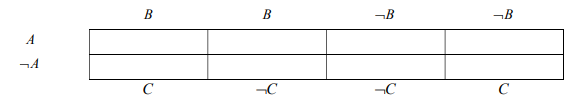
\includegraphics[width = 1 \linewidth]{kv-1.png}
        \caption{A figure caption}
    \end{figure}
    Die Randbeschriftungen müssen so gewählt werden, dass 2 benachbarte Zellen 
    sich genau in einer Aussage unterscheiden.
    \item Aus einer Wahrheitstabelle die Wahrheitswerte ablesen und in das Diagramm eintragen. Hier verwenden wir das Beispiel 16. Eine disjunktive Normalform kann an 
    der Wahrheitstabelle abgelesen werden und gleich in das Karnaugh-Veitch-Diagramm eingetragen werden. Am einfachsten trägt man zuerst die Wahrheitswerte 
    ein, die am wenigsten häufig auftreten, hier also die falsch-Werte
    \begin{figure}[H]
        \centering
        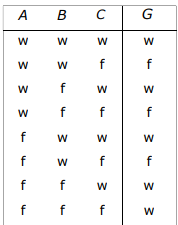
\includegraphics[width = .3 \linewidth]{kv-2.png}
        \caption{A figure caption}
    \end{figure}
    Nachdem die einen Wahrheitswerte vollständig eingetragen wurden (hier also 3 f-Werte), werden alle anderen Zellen auf den anderen Wahrheitswert gesetzt (hier 
    werden die 5 w-Werte ergänzt).
    \begin{figure}[H]
        \centering
        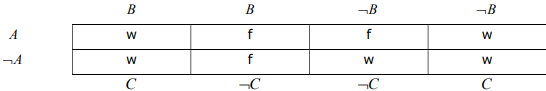
\includegraphics[width = 1 \linewidth]{kv-3.png}
        \caption{A figure caption}
    \end{figure}
    \item Blockbildung im Karnaugh-Veitch-Diagramm
    \begin{enumerate}
        \item Alle benachbarten w-Felder zu horizontalen oder vertikalen Blöcken zusammenfassen, die die Grösse einer 2er-Potenz besitzen.
        \item Hierbei gelten Zellen auch über den Rand als benachbart.
        \item Bei der MinTerm-Methode müssen alle w-Zellen durch solche Blöcke überdeckt werden, ohne dass eine f-Zelle überdeckt wird. Es können w-Zellen 
        mehrfach überdeckt werden. In dem Beispiel können wir den 4er-Block C
        und den 2er-Block \(\lnot A \land \lnot B\) nehmen und erhalten bei der Vereinfachung 
        mit dem Karnaugh-Veitch-Diagramm als Ergebnis
    \end{enumerate}
\end{enumerate}

\section{Beweise}
\begin{enumerate}
    \item Direkte Beweise \( A \implies B \)
    \item Indirekte Beweise \( \lnot B \implies \lnot A \)
    \item Widerspruchsbeweis = reductio ad absurdum \( A \land \lnot B \implies F \)
    \item Vollständige Induktion \( A(1) \land (A(n) \implies A(n+1)) \implies A(m),m \in \mathbb{N} \)
    \item Vollständige Fallunterscheidung \(A \leftrightarrow A_1 \lor \cdots A_n\) und es gilt \( (A_n \implies B) \) dann \( A \implies B \)
    \item Schubfachprinzip: Wenn n+1 Gegenstände (Objekte) auf n Schubladen (Kategorien) verteilt werden, dann befinden sich in mindestens einem Schubfach 2 Gegenstände
    \item Diagonalverfahren (Georg Cantor): Anzahl rationaler Zahlen ist genau so gross wie die Anzahl der natürlichen Zahlen. 
\end{enumerate}
\subsection{Vollständige Induktion}
\begin{enumerate}
    \item \textbf{Verankerung}: Es wird geprüft, ob \(A(n)\) für den ersten Wert stimmt.
    Ob also die Aussage \( A(n_0) \) gilt.
    \item \textbf{Induktionsschritt}: \(n \rightarrow n+1 \), Es wird gezeigt dass wenn \(A(n)\) gilt auch \(A(n+1)\) gilt. \( A(n) \implies A(n+1)\)
    \begin{enumerate}
        \item \textbf{Induktionsannahme}: \(A(n)\) sei richtig für \(n\)
        \item \textbf{Induktionsbehauptung}: \(A(n+1)\)
        \item \textbf{Induktionsbeweis}: Mit der Aussage \(A(n)\) die Richtigkeit der Behauptung \(A(n+1)\) zeigen.
    \end{enumerate}
\end{enumerate}
Für die Lösung von Induktionsbeweise können allen voran zwischen 4 gängigen Techniken gewählt werden.
Hier mit dem Beispiel \(f(n)=g(n)\):
\begin{enumerate}
    \item Direkter Beweis für einfache Fälle bspws. Fällen bei denen sich g(n) nicht vereinfachen lässt.
    \(f(n)=f_1(n)=f_m(n)=g(n)\)
    \item Differenz gleich Null für die Fälle, in denen die erste Technik zu kompliziert 
    scheint. \(f(n)-g(n)=0\)
    \item Äquivalenzumformungen für die Fälle, in denen auf der linken Seite 
    gleiche Faktoren (z.B. 6, oder (n+1) ) auftreten wie auf der rechten Seite.
    \item Dritte Grösse für die Fälle, in denen sich g(n) vereinfachen lässt (zum 
    Beispiel durch Ausmultiplizieren), nach dem Grundsatz "Sind zwei Grössen einer 
    dritten gleich, dann sind sie auch untereinander gleich".
\end{enumerate}

\subsection{Direkter Beweis}
Bei einem direkten Beweis wird die Behauptung aus den allgemein geltenden Grundlagen 
direkt abgeleitet. In der Sprache der Aussagenlogik können wir das so formulieren: Sei 
A(n) eine Aussage für eine natürliche Zahl n und B(n) eine Formel, die wahr ist, wenn 
A(n) wahr ist. Bei einem direkten Beweis versucht man also die Aussage \( A(n) \implies B(n)\)
direkt zu zeigen. 


\section{Axiome Natürlicher Zahlen}
\begin{equation}
    \parbox{30em}{
        \begin{enumerate}
            \item Null ist eine natürliche Zahl.
            \item Zu jeder natürlichen Zahl n gibt es genau einen Nachfolger n0, der auch eine 
            natürliche Zahl ist.
            \item Null ist nicht Nachfolger einer natürlichen Zahl. 
            \item Jede natürliche Zahl ist Nachfolger höchstens einer natürlichen Zahl.
            \item Die Menge der natürlichen Zahlen ist die kleinste Menge, die die Zahl Null und 
            mit jeder natürlichen Zahl auch ihren Nachfolger enthält.
        \end{enumerate}
    }
\end{equation}

\section{Sonstige Formeln}
\begin{equation}
    \text{Arithmetische Summenformel } \sum_{k=1}^{n}{k} = \frac{1}{2} n (n+1) \text{ for } n \in \mathbb{N}, n >= 1
\end{equation}
\begin{equation}
    \text{(Euklid) Die Menge der Primzahlen ist unendlich.}
\end{equation}

\section{Euklidischer Algorithmus}
\subsection{Erweiterter Euklidischer Algorithmus}